\documentclass[fleqn]{jbook}
\usepackage[dvips]{graphicx}
\usepackage{amsmath}
%%%%%%%%%%%%%%%%%%%%%%%%%%%%%%%%%%%%%%%%%%%%%%%%%%%%%%%%%%%%%%%%%%%%%%%%%%%%%%%%%%%%%%%%%%%%%

\begin{document}
\begin{question}{第5問}{}
放電管のスペクトルを調べるために、分光器を使って図\iref{2004phy5-3}のような実験を行った。放電管から出た発行は、凸レンズによって入り口スリット$S_1$上に集光される。$S_1$を通った光線は、凹面鏡1によって平行光線となり、回折格子$G$に入射する。回折光は凹面鏡2によって出口のスリット$S_2$上に集光されて、光電子増倍管によって検出される。$G$を回転することにより、$S_2$から出てくる光の波長を変化させることができる。

\begin{figure}[htbp]
\begin{center}
%\includegraphics[scale=0.4]{2004phy5-3.eps}
\includegraphics[width=10cm]{2004phys5_3.eps}
\caption{}
\ilabel{2004phy5-3}
\end{center}
\end{figure}

分光器の働きを理解するために、まず回折格子について考察する。回折格子の拡大図を図\iref{2004phy5-4}に示す。ただし、取り扱いを簡単にするために、溝の部分からの反射はまったくなく、平らな部分(反射面)の幅は溝に比べて十分に狭いと仮定する。入射光、回折光が回折格子の法線となす角度をそれぞれ$\alpha,\beta$、入射光の波長を$\lambda$、格子の間隔を$D$とする。$j=1,\ldots,N$は反射面の番号である。以下の設問に答えよ。

\begin{figure}[htbp]
\begin{center}
%\includegraphics[scale=0.4]{2004phy5-4.eps}
\includegraphics[width=7cm]{2004phys5_4.eps}
\caption{}
\ilabel{2004phy5-4}
\end{center}
\end{figure}

\begin{enumerate}

\item 十分遠方の点$P$における、$j$番目と$j+1$番目の反射面からの回折光の位相差$\phi$を求め、回折光が強くなるための条件を、$\alpha,\beta$を含む式で書け。ただし、空気の屈折率は1と考えてよい。

\item
$j=1$の反射面からの回折光の点$P$における電場が、複素表示で

$$
E=E_0 \exp(i\omega t)
$$
と与えられるとして、$N$本の反射面からの回折光をたし合わせた電場$E_{\text{tot}}$を、$\phi$を含む複素表示で書け。ただし、$E_0$は$\alpha,\beta$によらないものとする。

\item
点$P$における蛍雪高強度は$|E_{\text{tot}}|^2$に比例する。$|E_{\text{tot}}|^2$の$\phi=2\pi$近傍でのふるまいを、$\phi$の関数として図示せよ。なお、最大値及び、極大、極小などの特徴的な点の$\phi$座標を記入すること。

\end{enumerate}

つぎに、図\iref{2004phy5-3}に示した実際の分光器に単色光を入射した場合について考察する。

\setcounter{enumi}{3}
\begin{enumerate}
\item
設問3で、$\phi=2\pi$のピークは一次回折光とよばれ、分光に利用される。回折格子$G$によって、ある一定の方向に回折された光は、凹面鏡2によって
$S_2$を含む平面AB上の1点に位相差なく集光されるものとする。はじめに、波長$\lambda$において1次の回折光が$S_2$に集光されるように$G$の角度を固定($\alpha,\beta$を固定することに対応)する。次に、入射する単色光の強度を一定に保ちながら$\lambda$をわずかに変化させ、$\lambda+\Delta\lambda$とする。このとき、$S_2$における光の強度を、$\Delta\lambda$の関数として、$\Delta\lambda\ge 0$の領域で図示し、最初に現れる極小点における$\Delta\lambda$の値を、mm単位で求めよ。ただし、波長$\lambda$を600nm、回折格子の1mmあたりの溝の本数を1000、回折格子の溝に垂直方向の幅を60nmとする。また、回折格子の全面が一様に回折に寄与しているとする。

\item
設問4で求めた最初の極小点における$\Delta\lambda$の値は、分光器のスペクトル分解能のめやすを与える。しかし、実際の分光器のスペクトル分解能は、スリット($S_1,S_2$)の幅にも依存する。その理由を簡潔に述べよ。
\item
この実験で光検知器として用いている「光電子増倍管」の原理を、簡潔に説明せよ。また、この光電子増倍管は図\iref{2004phy5-5}にしめすような波長感度特性を持っているが、短波長と長波長で感度がゼロに近づいていくのはなぜか。その理由を簡潔に説明せよ。\end{enumerate}
\begin{figure}[htbp]
\begin{center}
%\includegraphics[scale=0.4]{2004phy5-5.eps}
\includegraphics[width=9cm]{2004phys5_5.eps}
\caption{}
\ilabel{2004phy5-5}
\end{center}
\end{figure}
\end{question}

\begin{answer}{第5問}{}
\begin{enumerate}

\item
$j$番目と$j+1$番目の反射面からの回折光の光路差は$D(\sin \alpha - \sin \beta)$で与えられるから、求める位相差$\phi$は
\begin{equation}
\phi =2\pi \times \frac{D(\sin \alpha - \sin \beta)}{\lambda}
\end{equation}
また、$n$を整数とすると回折光が強くなる条件は、
\begin{equation}
D(\sin \alpha - \sin \beta) =n\lambda
\end{equation}

%%%%%%%%%%%%%%%%%%%%%%%%%%%%%%

\item
$j$番目の反射面からの回折光の点Pにおける電場は
\begin{equation}
E_j =E_0 \exp \{i\omega t-i(j-1)\phi \}
\end{equation}
と書けるから、
\begin{equation}
\begin{split}
E_{tot}&=\sum ^{N-1}_{j=0}E_j =\sum ^{N-1}_{j=0}E_0 \exp (i\omega t -ij\phi) \\
       &=E_0 \exp (i\omega t)\frac{1-e^{-iN\phi}}{1-e^{-i\phi}}
\end{split}
\end{equation}



%%%%%%%%%%%%%%%%%%%%%%%%%%%%%%

\item
前問の結果より、
\begin{equation}
\begin{split}
|E_{tot}|^2&=|E_0|^2 
\frac{(1-e^{iN\phi})(1-e^{-iN\phi})}{(1-e^{i\phi})(1-e^{-i\phi})} \\
         &=|E_0|^2\frac{1-\cos N\phi }{1-\cos \phi} \\
         &=|E_0|^2\left(\frac{\sin \frac{N\phi}{2}}{\sin \frac{\phi}{2}}\right)^2
\end{split}
\end{equation}
となるから、$|E_{tot}|^2$の$\phi =2\pi$近傍での振舞いは下図のようになる。

\begin{figure}[h]
\begin{center}
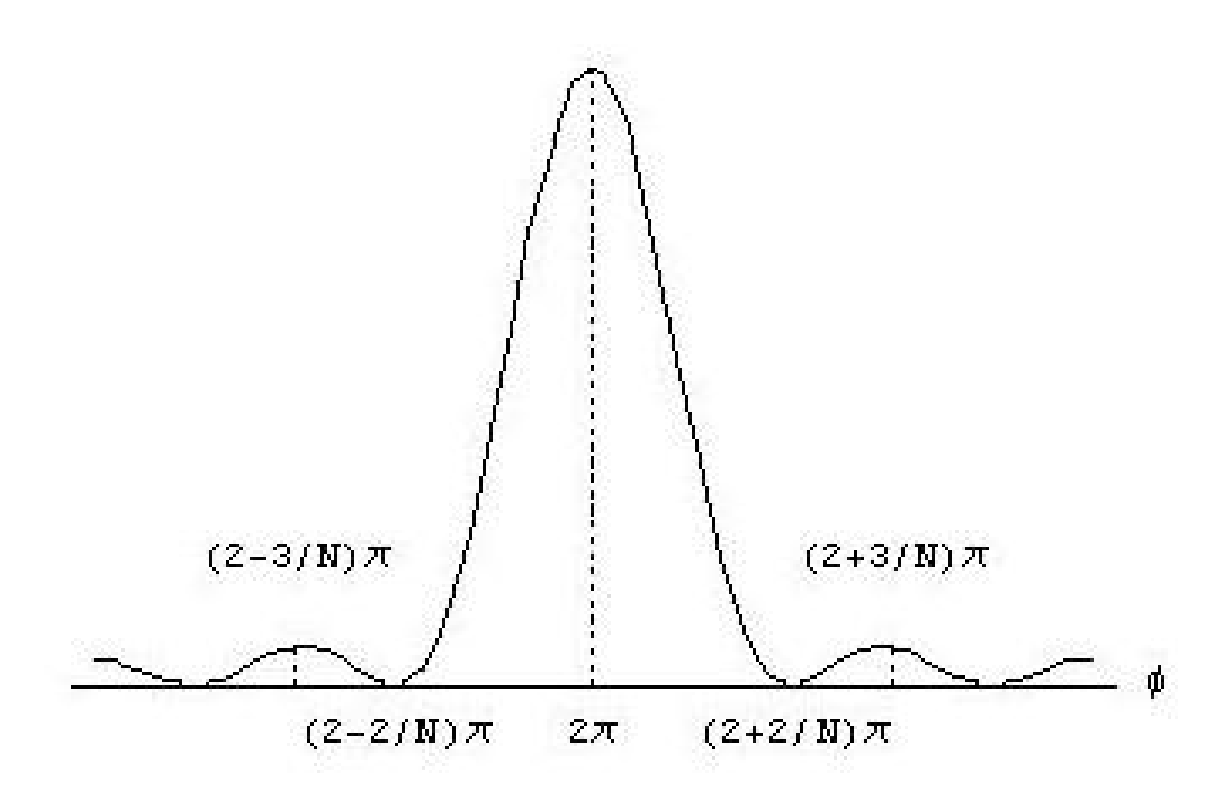
\includegraphics[width=6.0cm,clip]{2004phy5-1.eps}
\caption{}
\ilabel{gas}
\end{center}
\end{figure}

%%%%%%%%%%%%%%%%%%%%%%%%%%%%%%

\item

\begin{equation}
\phi (\Delta \lambda)=2\pi 
\times \frac{D(\sin \alpha - \sin \beta)}{\lambda +\Delta \lambda} 
=\frac{2\pi C}{\lambda +\Delta \lambda}
\end{equation}
とおくと、一次回折光では$\phi (0)=2\pi$より$C=\lambda$である。

回折格子の全面が一様に回折に寄与することから、$S_2$における光の強度を
$I(\Delta \lambda)$とおくと、
\begin{equation}
I(\Delta \lambda)\propto |E_{tot}|^2=|E_0|^2 
\frac{\sin \frac{N\phi}{2}}{\sin \frac{\phi}{2}}
\end{equation}
であるから、Aを定数として
\begin{equation}
I(\Delta \lambda)=A\left[\frac{\sin \frac{N\pi}{1+\frac{\Delta \lambda}{\lambda}}}{\sin \frac{\pi}{1+\frac{\Delta \lambda}{\lambda}}}\right]^2
\eqname{intensity}
\end{equation}
と書ける。\eqhref{intensity}式に$N=60000、\lambda =600nm$を代入し、
$I(\Delta \lambda)$を図示すると図のようになる。

\begin{figure}[htpb]
\begin{center}
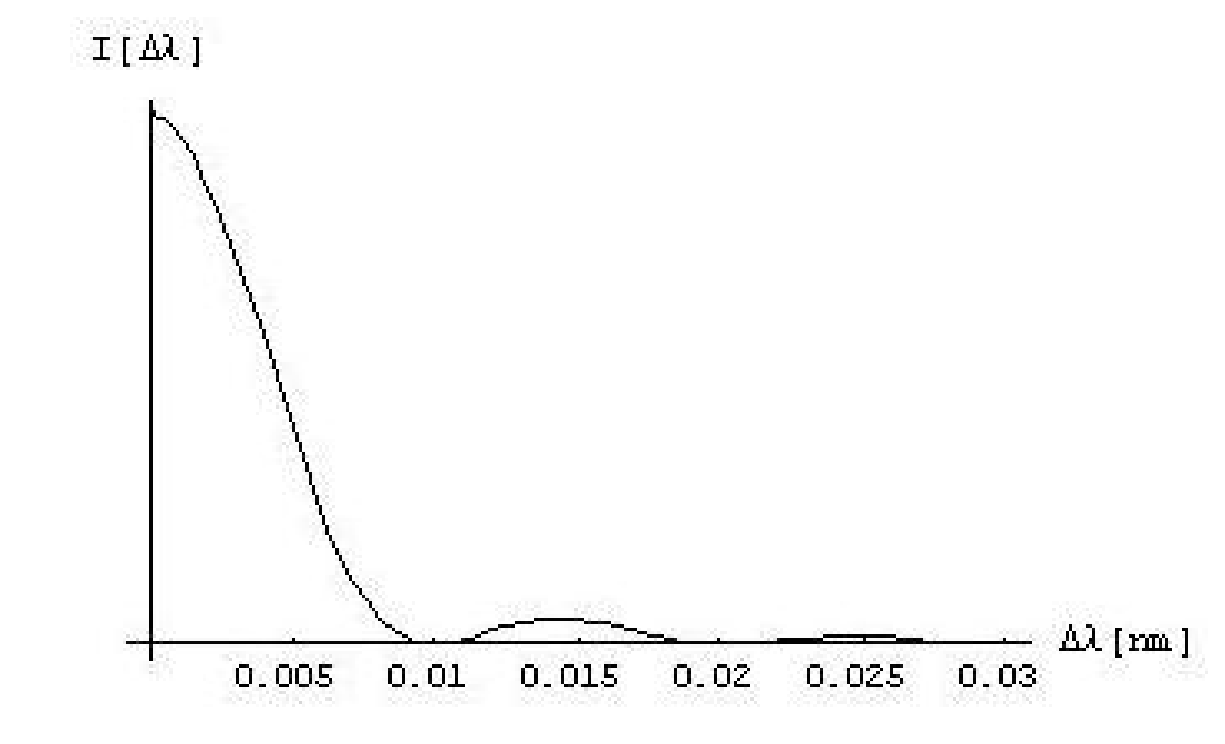
\includegraphics[width=6.0cm,clip]{2004phy5-2.eps}
\caption{}
\ilabel{lambda}
\end{center}
\end{figure}


また、最初に極小点が現れるとき、3.の結果より
\begin{equation}
\frac{\pi}{1+\frac{\Delta \lambda}{\lambda}}=(1-\frac{1}{N})\pi
\end{equation}
であるからこれを解いて
\begin{equation}
\Delta \lambda =\frac{1}{N-1}\lambda =1.0 \times 10^{-2} nm
\end{equation}
%%%%%%%%%%%%%%%%%%%%%%%%%%%%%%

\item 

スリット$S_1$と$S_2$においても回折が起こり、光が広がるため。
%%%%%%%%%%%%%%%%%%%%%%%%%%%%%%

\item
\begin{description}
\item[光電子増倍管の原理]
光子が光電面に当たると、光電効果により電子を放出する。放出された電子は電場によって加速され、ダイノードをたたく。このときダイノードより多数の電子が放出される。この放出された電子は次のダイノードとの間にかけられた電場によって加速され、次のダイノードに当たり、さらに多くの電子を放出する。これを繰り返し、一つの光子から多数の電子が生成され、電流として観測する。

\item[波長感度特性]
長波長の光子に対する感度は主に光電陰極の光の吸収の減少と光電子に与えられるエネルギーの減少で決められる。波長が長くなると光電子は光電陰極の表面から離脱することのできるエネルギーを持たなくなり、感度はゼロに近づく。

一方、短波長側の応答は光が光電子放出層に到達するまでに通過する窓の性質によって決まる。窓の遮断波長より短い光に対しては感度が悪くなる。
\end{description}

\end{enumerate}
\end{answer}
\end{document}
